\chapter{Validaci'on del M'etodo de la Ecuaci'on de Boltzmann en Redes}



\section{Introducci'on}

En este ap'endice presentamos brevemente la simulaci'on num'erica 
usando el m'etodo de la ecuaci'on de Boltzmann en redes (EBR) de  tres
flujos que nos ayudan a validar el c'odigo con el cual se realizan simulaciones num'ericas
de la levitaci'on ac'ustica.
En el primer problema, presentado en la secci'on~\ref{sec:hugoniot}, medimos la velocidad de propagaci'on de 
las ondas de choque formadas en un tubo unidimensional con dos zonas de densidad diferentes. Las
ondas de choque aparecen en fluidos compresibles y viajan a velocidades supers'onicas.
En la secci'on~\ref{sec:couette}, presentamos la interacci'on de una part'icula circular s'olida
libre de moverse colocada en  el centro de un flujo de Couette. El torque ejercido
por el perfil de velocidades sobre la part'icula hace que 'esta alcance una velocidad
angular constante que a su vez es funci'on del n'umero de Reynolds.
El 'ultimo problema, presentado en la secci'on~\ref{sec:sedimentacion}, es el de una part'icula solida
circular que se sedimenta en una cavidad bajo la acci'on de una fuerza de cuerpo. 
La din'amica del movimiento de la part'icula
es funci'on del n'umero de Reynolds. 
Todos los resultados los obtenemos usando el m'etodo de la ecuaci'on de Boltzmann en 
redes y  los comparamos con los reportados 
en la literatura. Encontramos que hay un acuerdo entre nuestros resultados y los reportados
en la literatura.



\section{Onda de choque en una cavidad}
\label{sec:hugoniot}



\begin{figure}
\centering
%\begin{pspicture}(8,2)
%%\psgrid
%\psframe(0,.6)(4,2)
%\psframe(4,.6)(8,2)
%\rput[C](2,1.3){$\rho_{+}$}
%\rput[C](6,1.3){$\rho_{-}$}
%\psline{<->}(0,.2)(8,.2)
%\rput[C](4,-.1){$L_x$}
%\end{pspicture}
\caption{\label{fig:esquema-hugoniot}
Esquema del tubo bidimensional con la mitad izquierda a $\rho_+$ y la mitad derecha a $\rho_-$
donde $\rho_+ > \rho_-$ y de largo $L_x$. }
\end{figure}



Se puede obtener una onda de choque si en un tubo  cerrado en los extremos izquierdo y derecho y con
condiciones peri'odicas a la frontera en la direcci'on vertical, como el que mostramos
en la figura~\ref{fig:esquema-hugoniot},  establecemos la densidad 
del lado izquierdo en $\rho_+$, y la
del lado derecho en $\rho_-$ para $t<0$ y $\rho_+>\rho_-$. El fluido contenido en el tubo se encuentra
inicialmente en reposo y al retirar la pared central para $ t \geq 0$ 
se forman dos frentes de ondas, una onda de choque que viaja 
hacia la derecha con velocidad supers'onica $v_s$ y una onda de rarefacci'on que  
viaja en la direcci'on opuesta con velocidad subs'onica. 
Al avanzar la onda de choque y la onda de rarefacci'on,
la densidad entre las ondas alcanza un valor $\rho_c$. 
Estos valores los podemos calcular con las relaciones de Rankine--Hugoniot~\cite{ansumali00},
\begin{equation}
v_s^2 = r_cc_s^2, \qquad \rho_c = r_c\rho_- \qquad{\text y}\qquad u_c=\frac{r_c-1}{\sqrt{r_c}}c_s,
\end{equation}
donde $c_s$ es la velocidad del sonido, $v_s$ es la velocidad de la onda supers'onica que viaja
hacia la derecha, $\rho_c$ es la densidad en el centro entre los frentes de compresi'on
y rarefacci'on y $u_c$ es la velocidad a la que crece la zona central. Adem'as $r_c$ es la soluci'on de
\begin{equation} \label{ec:logr}
\log r_c + \log \frac{r_c-1}{\sqrt{r_c}} = \log \frac{\rho_+}{\rho_-}.
\end{equation}

\begin{figure}
%%GNUPLOT: LaTeX picture with Postscript
%\begin{picture}(0,0)%
%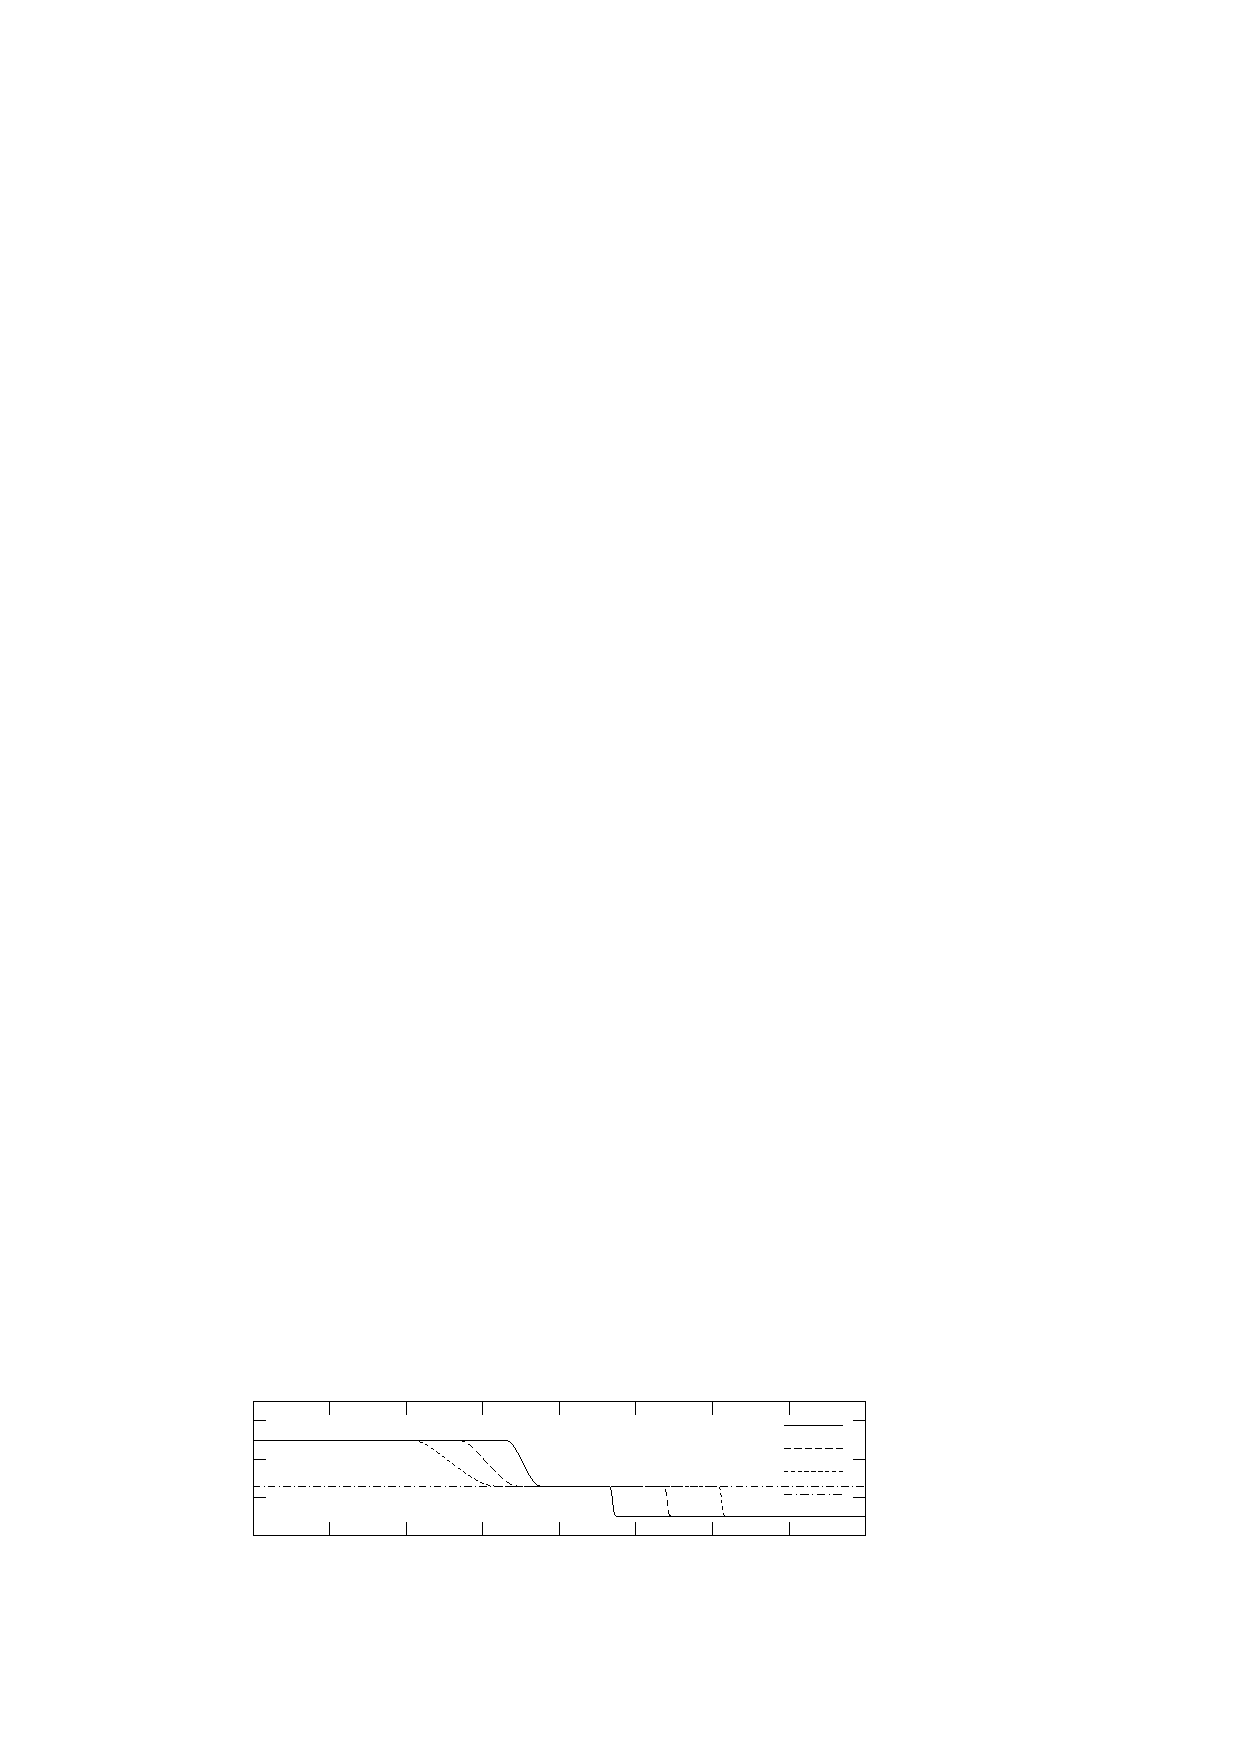
\includegraphics{rankine-densidad}%
%\end{picture}%
%\begingroup
%\setlength{\unitlength}{0.0200bp}%
%\begin{picture}(18000,5400)(0,0)%
%\put(2200,1650){\makebox(0,0)[r]{\strut{} 0.2}}%
%\put(2200,2564){\makebox(0,0)[r]{\strut{} 0.4}}%
%\put(2200,3479){\makebox(0,0)[r]{\strut{} 0.6}}%
%\put(2200,4393){\makebox(0,0)[r]{\strut{} 0.8}}%
%\put(2475,1100){\makebox(0,0){\strut{} 0}}%
%\put(4313,1100){\makebox(0,0){\strut{} 100}}%
%\put(6150,1100){\makebox(0,0){\strut{} 200}}%
%\put(7988,1100){\makebox(0,0){\strut{} 300}}%
%\put(9825,1100){\makebox(0,0){\strut{} 400}}%
%\put(11663,1100){\makebox(0,0){\strut{} 500}}%
%\put(13500,1100){\makebox(0,0){\strut{} 600}}%
%\put(15338,1100){\makebox(0,0){\strut{} 700}}%
%\put(17175,1100){\makebox(0,0){\strut{} 800}}%
%\put(550,3250){\rotatebox{90}{\makebox(0,0){\strut{}$\rho$}}}%
%\put(9825,275){\makebox(0,0){\strut{}$x$}}%
%\put(14950,4275){\makebox(0,0)[r]{\strut{}$t=100$}}%
%\put(14950,3725){\makebox(0,0)[r]{\strut{}$t=200$}}%
%\put(14950,3175){\makebox(0,0)[r]{\strut{}$t=300$}}%
%\put(14950,2625){\makebox(0,0)[r]{\strut{}$\rho_c$}}%
%\end{picture}%
%\endgroup
%\endinput

\caption{\label{fig:rank-dens} Evoluci'on temporal del perfil de densidad. Para las condiciones
iniciales de este problema $r_c=0.457539$, $v_s = 0.712$ y $\rho_c=0.457539$ .}
\end{figure}

Realizamos simulaciones num'ericas usando el m'etodo de la ecuaci'on de Boltzmann
en redes para el problema descrito anteriormente. Simulamos un tubo  de $L_x= 800$ nodos
de longitud y altura $L_y=10$, $\tau=0.7$, con densidades $\rho_+=0.7$ y $\rho_-=0.3$ en las mitades izquierda
y derecha, respectivamente. Las paredes izquierda y derecha las simulamos usando el rebote hacia atr'as, aunque
en los resultados presentados la onda de choque no alcanza a rebotar en la pared.
En la figura~\ref{fig:rank-dens} observamos  dos frentes de onda viajando en direcciones opuestas  para 
diferentes tiempos y  $\rho_c=0.457539$ es el predicho
por la teor'ia. Para verificar que el frente de choque avanza con velocidad supers'onica $v_s$ 
en la figura~\ref{fig:rank-vs} mostramos  el valor de la densidad en la posici'on $x-v_st$, 
para tres valores de $t$. 
\begin{figure}
%%GNUPLOT: LaTeX picture with Postscript
%\begin{picture}(0,0)%
%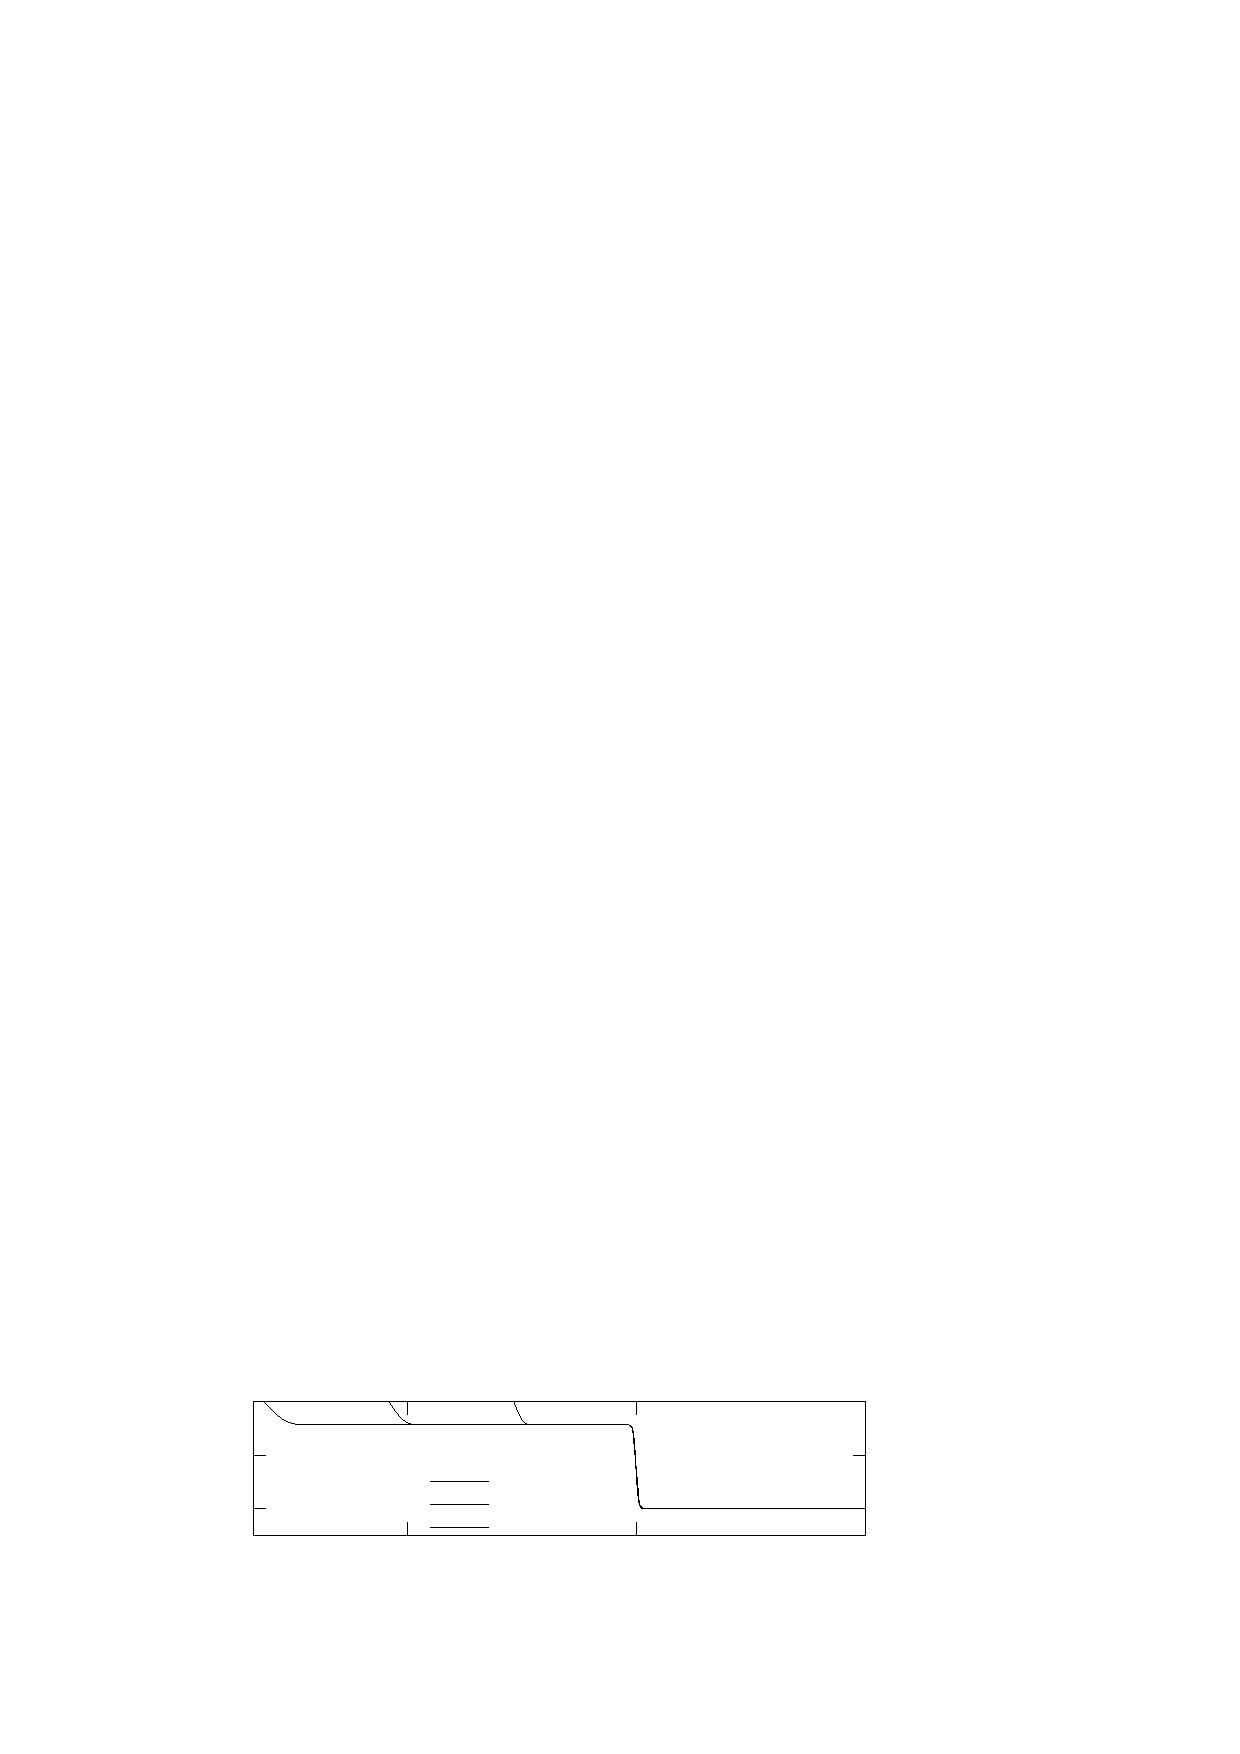
\includegraphics{rankine-vs}%
%\end{picture}%
%\begingroup
%\setlength{\unitlength}{0.0200bp}%
%\begin{picture}(18000,5400)(0,0)%
%\put(2200,2290){\makebox(0,0)[r]{\strut{} 0.3}}%
%\put(2200,3570){\makebox(0,0)[r]{\strut{} 0.4}}%
%\put(2200,4850){\makebox(0,0)[r]{\strut{} 0.5}}%
%\put(6184,1100){\makebox(0,0){\strut{} 200}}%
%\put(11680,1100){\makebox(0,0){\strut{} 400}}%
%\put(17175,1100){\makebox(0,0){\strut{} 600}}%
%\put(550,3250){\rotatebox{90}{\makebox(0,0){\strut{}$\rho$}}}%
%\put(9825,275){\makebox(0,0){\strut{}$x$}}%
%\put(689,-1548){\makebox(0,0)[l]{\strut{}(null)}}%
%\put(6459,2930){\makebox(0,0)[r]{\strut{}$t=100$}}%
%\put(6459,2380){\makebox(0,0)[r]{\strut{}$t=200$}}%
%\put(6459,1830){\makebox(0,0)[r]{\strut{}$t=300$}}%
%\end{picture}%
%\endgroup
%\endinput

\caption{\label{fig:rank-vs} Cada perfil de puntos representa   $x - v_st$,
donde $v_s$ es la velocidad de avance del frente supers'onico
 y $t$ es  el tiempo transcurrido desde el comienzo del experimento. 
Para este caso $v_s=\sqrt{r_c}c_s=0.712$}
 \end{figure}





\section{Cilindro suspendido en un flujo Couette}
\label{sec:couette}

Se sumerge un cilindro con la misma densidad que el fluido en   el centro de un canal horizontal
con  condiciones peri'odicas en las fronteras en el eje horizontal, como 
mostramos esquem'aticamente en la figura~\ref{fig:couette}. Las paredes superior e inferior
se mueven en direcciones opuestas. El canal tiene una altura $h=5D$ y de largo $2h$, donde
$D$ es el di'ametro de la part'icula suspendida. El n'umero adimensional $Re$
se define como
\begin{equation}\label{Re_c}
Re=\frac{\gamma D^2}{\nu},
\end{equation}
donde $\gamma=2U_p/h$ es la raz'on de corte definida como la velocidad de la pared $U_p$ entre la altura 
del canal y $\nu$  es la viscosidad del fluido.
Si el cilindro, libre de moverse, se encuentra en el centro del canal y su densidad es la misma
que la del fluido, 'este comenzar'a a aumentar su velocidad
angular hasta alcanzar  $\omega^\ast=\omega/\gamma= 0.5$ para 
valores de $Re \ll 1$  y disminuye conforme se aumenta el n'umero $Re$. 


\begin{figure}
%
%\centering
%\begin{pspicture}(10,5)
%%\psgrid
%\psline[linewidth=1mm](0,0)(10,0)
%\psline[linewidth=1mm](0,5)(10,5)
%\psline{->}(3,4.5)(7,4.5)
%\psline{<-}(3,0.5)(7,0.5)
%\psline{<->}(.4,.2)(.4,4.8)
%\pscircle(5,2.5){1.}
%\psarc{<-}(5,2.5){1.3}{270}{0} 
%\rput[C](6.5,2.6) {$\omega$}
%\rput[C](5,4.7) {$u_w$}
%\rput[C](5,.7) {$u_w$}
%\rput[C](.6,2.5) {$h$}
%\psline{<->}(0,-.6)(10,-.6)
%\rput[C](5,-1){$2h$}
%\end{pspicture}

\vskip 1cm
\caption{\label{fig:couette}
Esquema del problema de un cilindro infinito suspendido en un flujo cortante. El cilindro
tiene un di'ametro D, y la cavidad tiene una altura $h=5D$ y $2h$ de ancha. El cilindro
se coloca en el centro de la cavidad.
}
\end{figure}


Este problema lo resolvemos usando el m'etodo de la EBR y comparamos con los resultados experimentales obtenidos por 
Poe {\it et al}~\cite{poe75}, qui'en coloc'o un cilindro en un flujo cortante y midi'o su 
velocidad angular terminal, como mostramos en la figura~\ref{fig:w} para diferentes valores de $Re$. 
Las simulaciones num'ericas las realizamos en una malla de $95 \times 190$, $D=19$  y $\tau=0.6$. Los resultados
obtenidos usando el m'etodo de la EBR no se alejan m'as de un 5\% de los valores encontrados experimentalmente.
\begin{figure}
%%GNUPLOT: LaTeX picture with Postscript
%\begin{picture}(0,0)%
%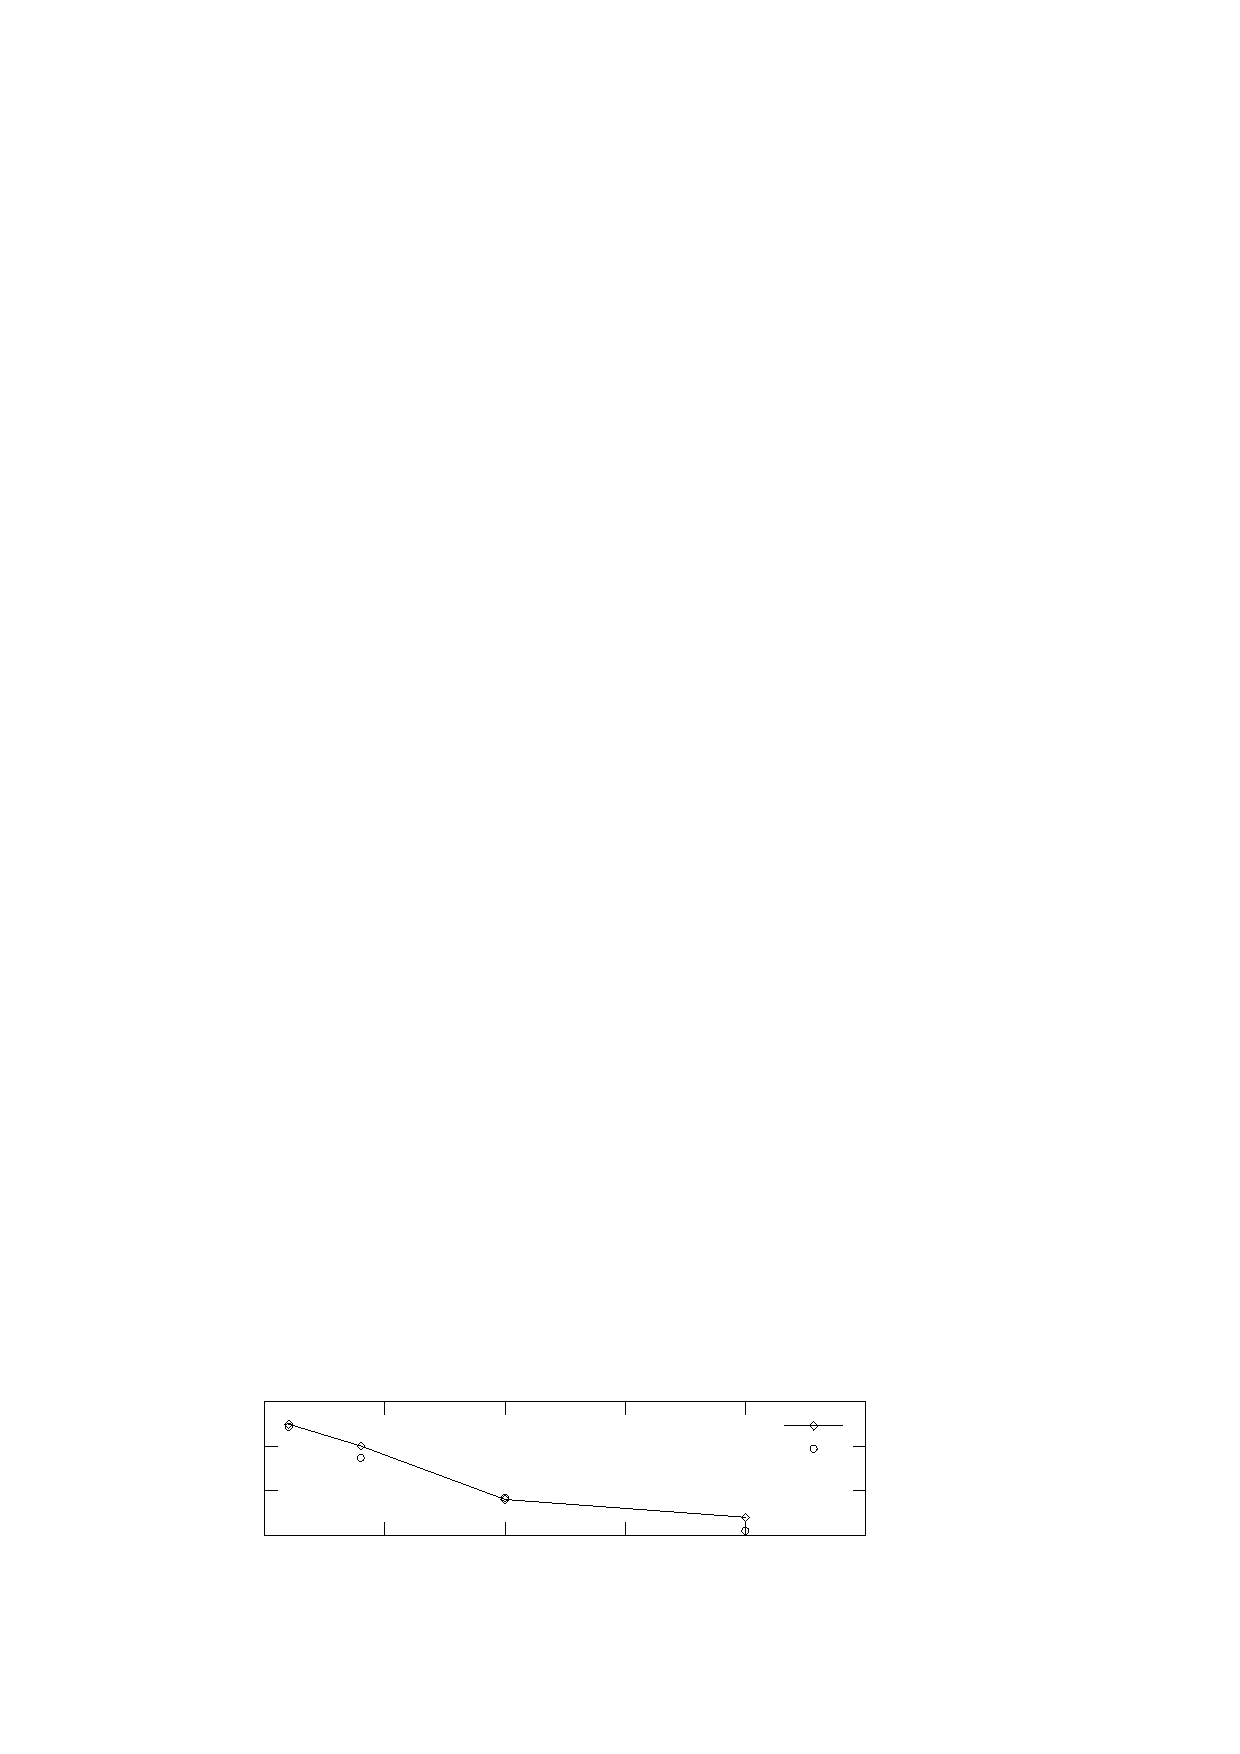
\includegraphics{angular}%
%\end{picture}%
%\begingroup
%\setlength{\unitlength}{0.0200bp}%
%\begin{picture}(18000,5400)(0,0)%
%\put(2475,1650){\makebox(0,0)[r]{\strut{}0.425}}%
%\put(2475,2717){\makebox(0,0)[r]{\strut{}0.450}}%
%\put(2475,3783){\makebox(0,0)[r]{\strut{}0.475}}%
%\put(2475,4850){\makebox(0,0)[r]{\strut{}0.500}}%
%\put(2750,1100){\makebox(0,0){\strut{} 0}}%
%\put(5635,1100){\makebox(0,0){\strut{} 1}}%
%\put(8520,1100){\makebox(0,0){\strut{} 2}}%
%\put(11405,1100){\makebox(0,0){\strut{} 3}}%
%\put(14290,1100){\makebox(0,0){\strut{} 4}}%
%\put(17175,1100){\makebox(0,0){\strut{} 5}}%
%\put(550,3250){\rotatebox{90}{\makebox(0,0){\strut{}$\Omega/\gamma$}}}%
%\put(9962,275){\makebox(0,0){\strut{}$Re$}}%
%\put(14950,4275){\makebox(0,0)[r]{\strut{}Poe {\it et al}}}%
%\put(14950,3725){\makebox(0,0)[r]{\strut{}EBR}}%
%\end{picture}%
%\endgroup
%\endinput

\caption{\label{fig:w} 
Velocidad angular adimensional para diferentes valores de $Re$. Los experimentos num'ericos
se llevaron a cabo en una cavidad con condiciones peri'odicas en las fronteras izquierda y derecha.
La relaci'on de aspecto $h/D = 5$, donde $h$ es la altura de la cavidad y $D$ el di'ametro de la
part'icula.
}
\end{figure}



\begin{figure}
%%GNUPLOT: LaTeX picture with Postscript
%\begin{picture}(0,0)%
%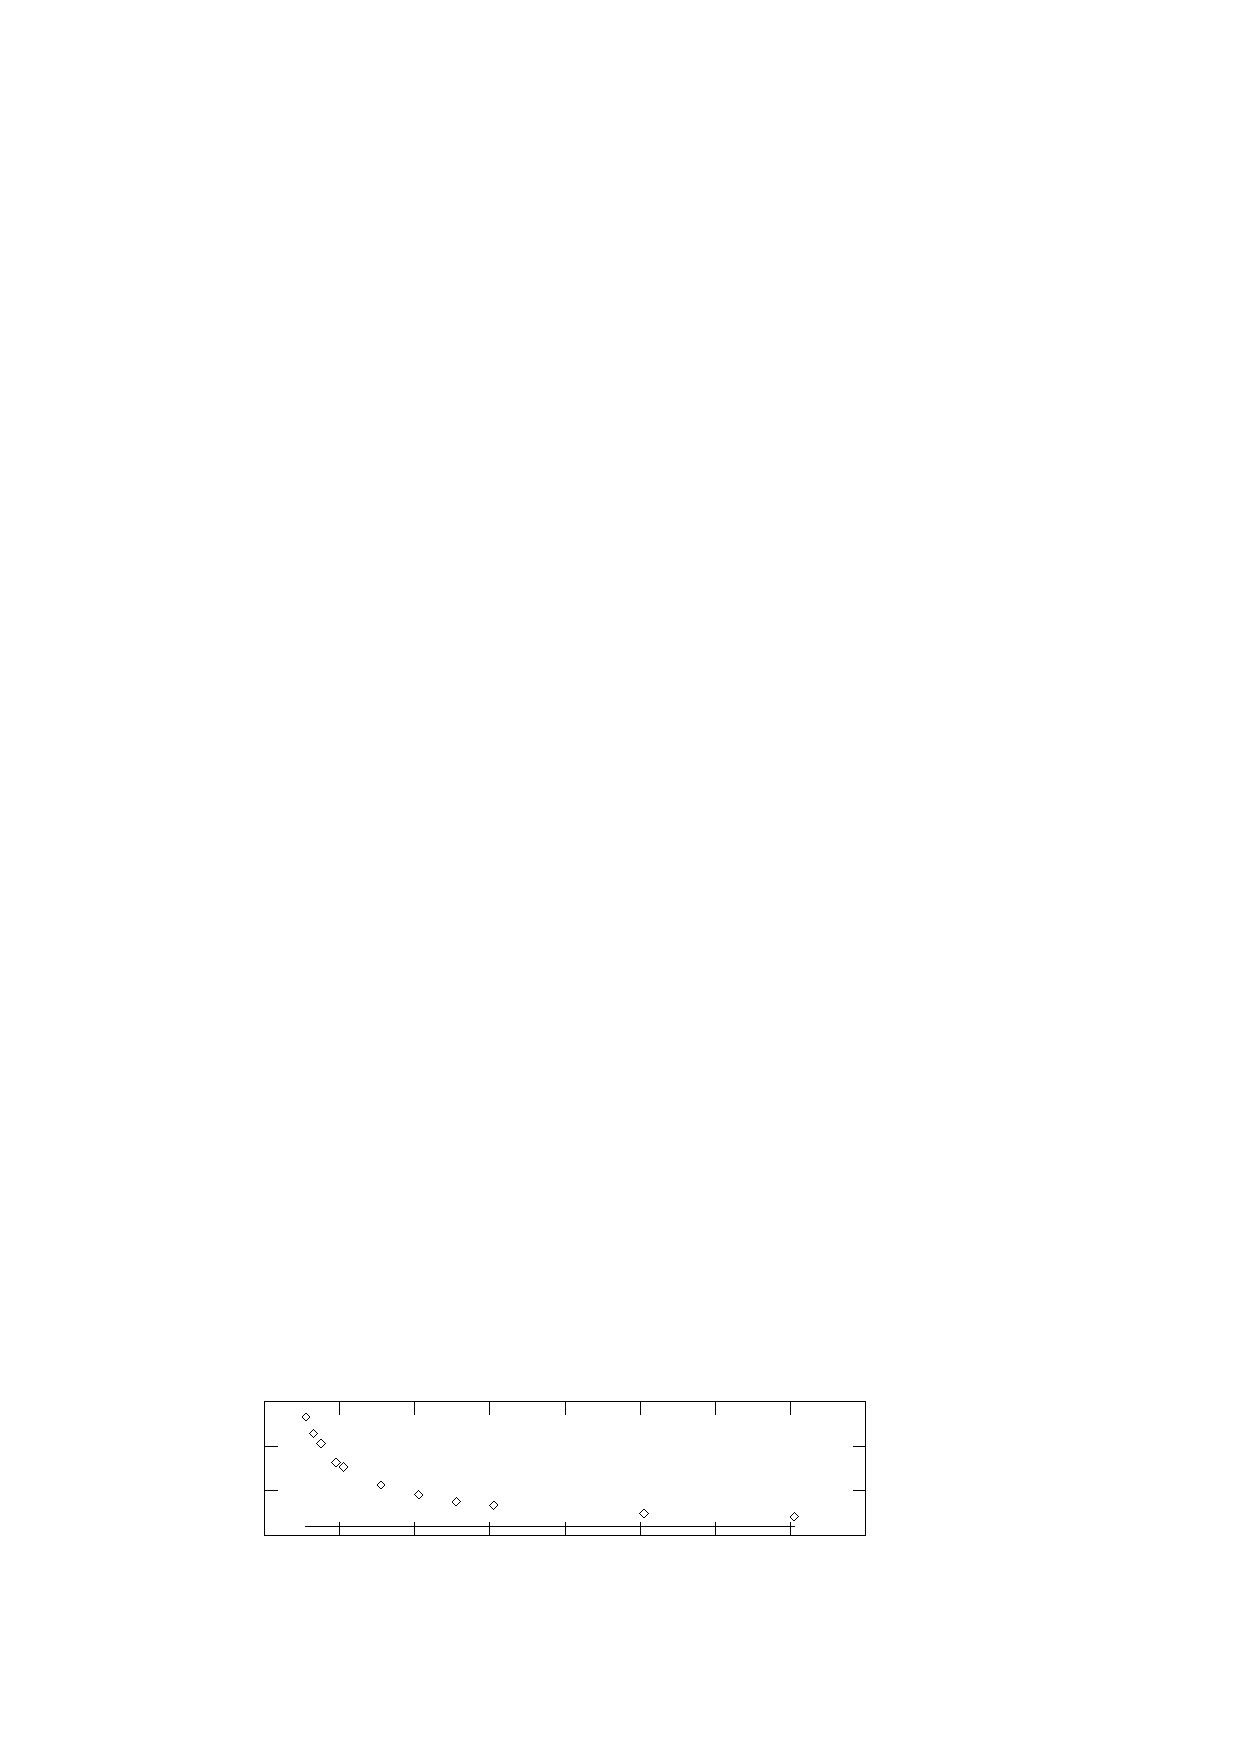
\includegraphics{Re0_187-Hr8}%
%\end{picture}%
%\begingroup
%\setlength{\unitlength}{0.0200bp}%
%\begin{picture}(18000,5400)(0,0)%
%\put(2475,1650){\makebox(0,0)[r]{\strut{}0.480}}%
%\put(2475,2717){\makebox(0,0)[r]{\strut{}0.490}}%
%\put(2475,3783){\makebox(0,0)[r]{\strut{}0.500}}%
%\put(2475,4850){\makebox(0,0)[r]{\strut{}0.510}}%
%\put(2750,1100){\makebox(0,0){\strut{} 0}}%
%\put(4553,1100){\makebox(0,0){\strut{} 10}}%
%\put(6356,1100){\makebox(0,0){\strut{} 20}}%
%\put(8159,1100){\makebox(0,0){\strut{} 30}}%
%\put(9963,1100){\makebox(0,0){\strut{} 40}}%
%\put(11766,1100){\makebox(0,0){\strut{} 50}}%
%\put(13569,1100){\makebox(0,0){\strut{} 60}}%
%\put(15372,1100){\makebox(0,0){\strut{} 70}}%
%\put(17175,1100){\makebox(0,0){\strut{} 80}}%
%\put(550,3250){\rotatebox{90}{\makebox(0,0){\strut{}$\Omega/\gamma$}}}%
%\put(9962,275){\makebox(0,0){\strut{}$r$}}%
%\put(16372,4083){\makebox(0,0)[r]{\strut{}(a)}}%
%\end{picture}%
%\endgroup
%\endinput

%%GNUPLOT: LaTeX picture with Postscript
%\begin{picture}(0,0)%
%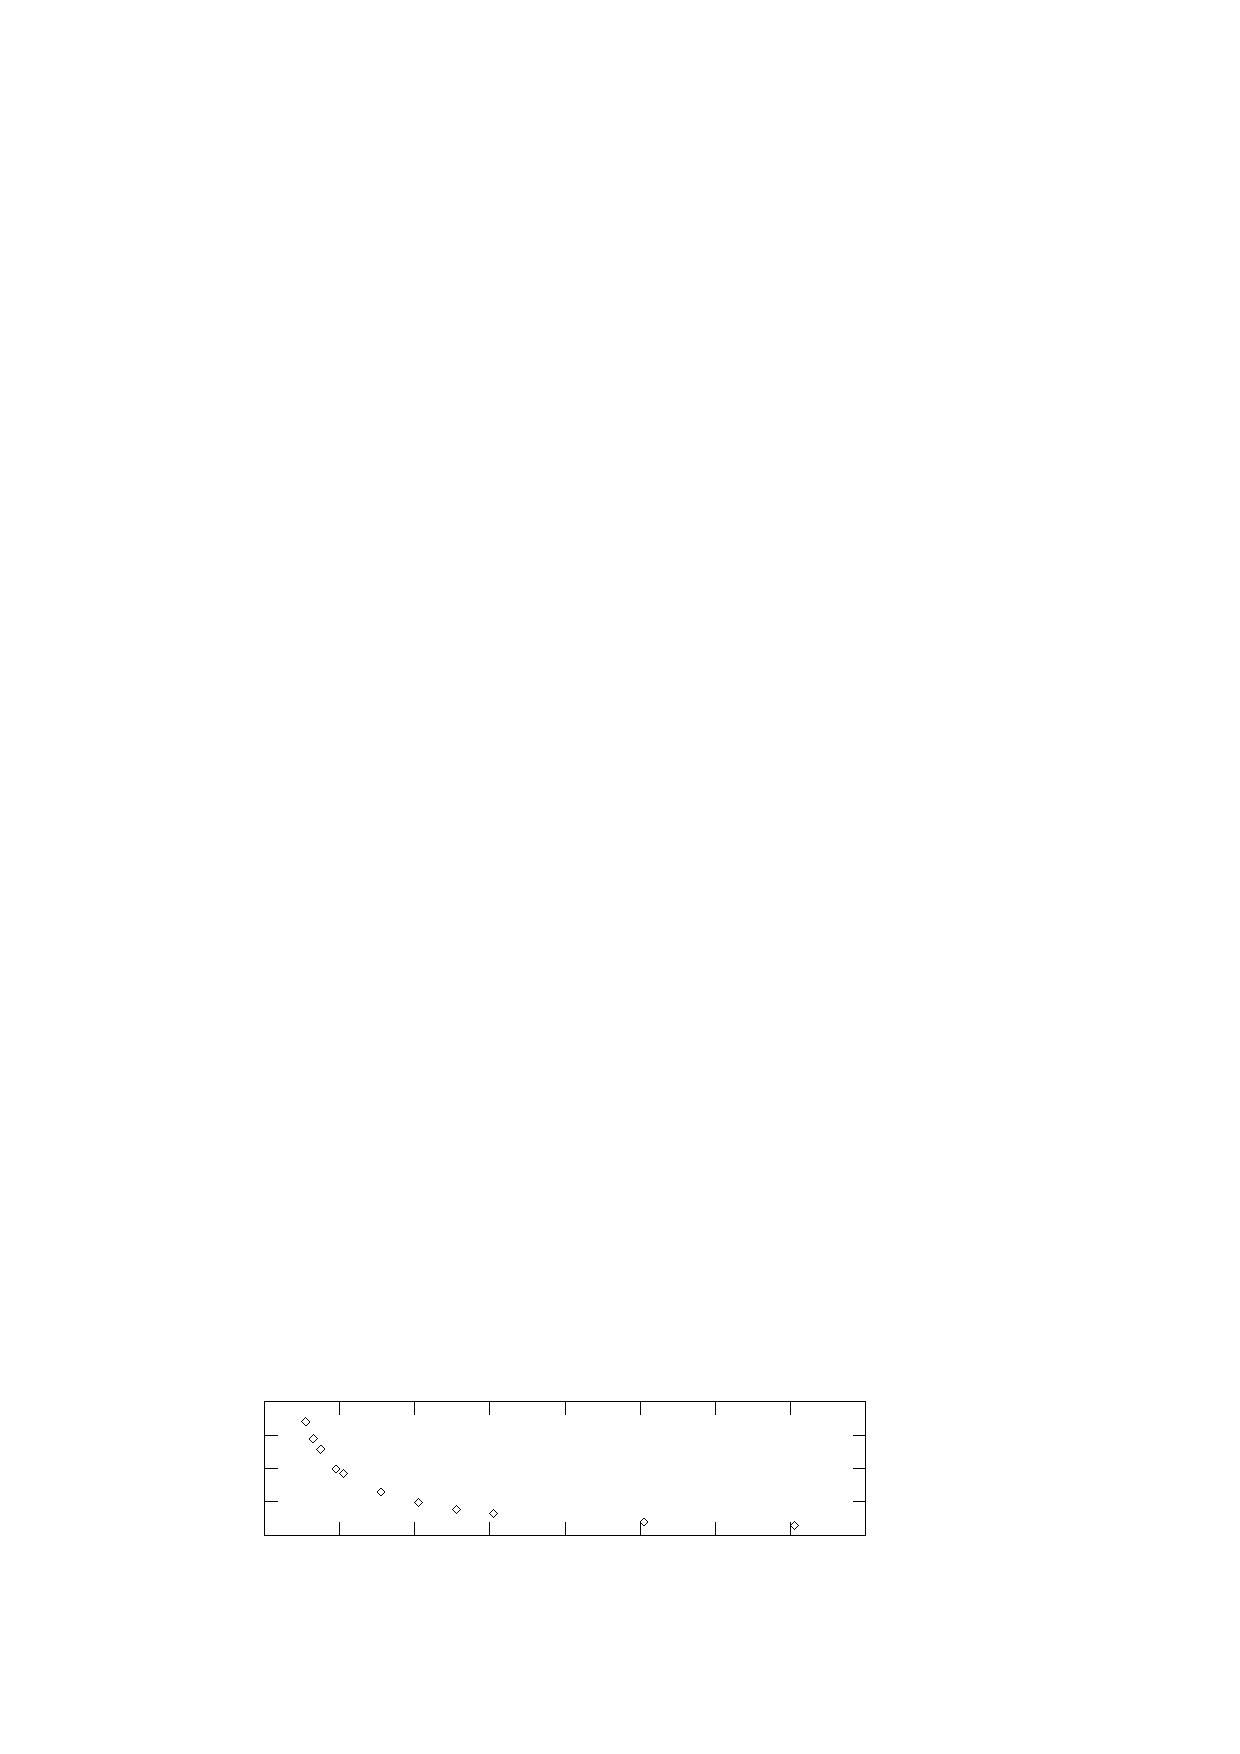
\includegraphics{error}%
%\end{picture}%
%\begingroup
%\setlength{\unitlength}{0.0200bp}%
%\begin{picture}(18000,5400)(0,0)%
%\put(2475,1650){\makebox(0,0)[r]{\strut{}0.000}}%
%\put(2475,2450){\makebox(0,0)[r]{\strut{}0.015}}%
%\put(2475,3250){\makebox(0,0)[r]{\strut{}0.030}}%
%\put(2475,4050){\makebox(0,0)[r]{\strut{}0.045}}%
%\put(2475,4850){\makebox(0,0)[r]{\strut{}0.060}}%
%\put(2750,1100){\makebox(0,0){\strut{} 0}}%
%\put(4553,1100){\makebox(0,0){\strut{} 10}}%
%\put(6356,1100){\makebox(0,0){\strut{} 20}}%
%\put(8159,1100){\makebox(0,0){\strut{} 30}}%
%\put(9963,1100){\makebox(0,0){\strut{} 40}}%
%\put(11766,1100){\makebox(0,0){\strut{} 50}}%
%\put(13569,1100){\makebox(0,0){\strut{} 60}}%
%\put(15372,1100){\makebox(0,0){\strut{} 70}}%
%\put(17175,1100){\makebox(0,0){\strut{} 80}}%
%\put(550,3250){\rotatebox{90}{\makebox(0,0){\strut{}error}}}%
%\put(9962,275){\makebox(0,0){\strut{}$r$}}%
%\put(16372,4083){\makebox(0,0)[r]{\strut{}(b)}}%
%\end{picture}%
%\endgroup
%\endinput

\caption{\label{fig:radios}
(a) Velocidad angular adimensional en funci'on del radio de la part'icula y
(b) error relativo escalado con  valor reportado por Poe {\it et al} 
para $Re= 0.187$ y $H=4D$ es $\Omega/\gamma=0.4820$, representado por la l'inea.
}
\end{figure}

Realizamos otro conjunto de experimentos manteniendo fijo el n'umero de Reynolds
en $Re=0.187$ y variamos el radio de la part'icula. Poe {\it et al}~\cite{poe75} reportaron
un valor de  $\Omega/\gamma=0.4820$ para este n'umero de Reynolds.  En la 
figura~\ref{fig:radios} (a) mostramos el valor de  $\Omega/\gamma$ en funci'on del radio de la
part'icula. Al aumentar el radio, la representaci'on de la part'icla en la malla $D2Q9$ es m'as
precisa y  por lo tanto los resultados mejoran. En la figura~\ref{fig:radios} (b) presentamos el
error relativo usando el valor reportado por Poe {\it et al}. Para un radio de part'icula
$r=70.5$ el error relativo es aproximadamente 0.01\% y para $r=9.5$ el error relativo es menor 
al 3\%. Para mantener la raz'on de aspecto de la cavidad, para $r=70.5$ los experimentos los realizamos
en una cavidad de $564 \times 282$ nodos. En esta cavidad, el problema se resuelve aproximadamente
en 26 horas de tiempo de c'omputo en un procesador AMD 64 2400 MHz. Para $r=9.5$, la cavidad
es de $152 \times 76$ nodos y se resuelve en aproximadamente 4 horas en el mismo procesador.  
Dado que el error relativo no es muy grande, y que la cavidad se resuelve en aproximadamente 
siete veces menos tiempo, escogimos un radio de $r=9.5$ para las simulaciones de la levitaci'on 
ac'ustica, y las demas dimensiones las escalamos para mantener las relaciones geom'etricas.




\section{Sedimentaci'on de una part'icula en una cavidad}
\label{sec:sedimentacion}

En una cavidad de ancho $W$ y alto $H$ colocamos una part'icula
de radio $r$ lejos de eje vertical del canal, como mostramos  esquem'aticamente en la  
figura~\ref{fig:scheme-sedimentacion},
y la dejamos sedimentar. La part'icula, m'as densa que el fluido,  cae bajo la acci'on de una fuerza de cuerpo y
su trayectoria depende del n'umero de Reynolds, definido como
\begin{equation}
Re=\frac{ur}{\nu},
\end{equation} 
donde $u$ es la velocidad terminal de la part'icula y $\nu$ la viscosidad del fluido. 
Otro factor importante es la relaci'on de aspecto del ancho de la cavidad entre 
el radio de la part'icula. Para los experimentos que presentamos a continuaci'on,
$W/r=4$.  La posici'on de la part'icula la adimensionalizamos con el ancho de la cavidad
\begin{equation}
x^\ast=\frac{x}{W},\qquad y^\ast=\frac{y}{W},
\end{equation}
donde $x$ y $y$ representan a la coordenada horizontal y vertical, respectivamente.

\begin{figure}
\centering
\vskip 1cm
%\begin{pspicture}(3,5)
%%\psgrid
%\psframe[](0.5,0)(2.5,5)
%\pscircle[fillstyle=solid,fillcolor=black] (1.2,4.5){.1}
%\psline[linewidth=0.1mm,linestyle=dashed] (1.5,0)(1.5,5)
%\psline{->}(2,2.5)(2,2)
%\rput[C](2,2.7) {$g$}
%\psline{<->}(0.5,5.3) (2.5,5.3)
%\psline{<->}(3,0)(3,5)
%\rput[C](1.5,5.4) {$W$}
%\rput[C](3.2,2.5){$H$}
%\end{pspicture}
\caption{\label{fig:scheme-sedimentacion}
Esquema del problema de sedimentaci'on en una cavidad de ancho $W=4r$ y alto $H$. 
La part'icula, inicialmente
en reposo,  se coloca lejos del centro horizontal en la parte superior de la cavidad. La part'icula
se sedimenta bajo la acci'on de una fuerza de cuerpo externa.
}
\end{figure}



Este problema ha sido resuelto num'ericamente por Feng {\it et al}~\cite{feng94} usando simulaci'on
directa para un amplio rango de valores del n'umero de Reynolds. Feng {\it et al} reportaron la existencia de cuatro reg'imenes  
identificados por el n'umero de Reynolds~\cite{feng94}. En el primer r'egimen, $0<Re<3.0$, la
part'icula s'olida se acerca suavemente hacia el centro de la part'icula, como 
vemos en la figura~\ref{fig:regimen-1-sedimentacion}. En el segundo r'egimen ,$3<Re<Re_{c}$, el
centro del canal contin'ua siendo el punto de equilibrio pero ahora, la part'icula
oscila alrededor del centro antes de alcanzar una posici'on de equilibrio, como 
observamos en la figura~\ref{fig:regimen-2-sedimentacion}. Cuando la part'icula alcanza un 
Reynolds cr'itico $Re_c$, la posici'on de equilibrio en el centro de la cavidad se vuelve
inestable y la part'icula oscila alrededor de esta posici'on, como vemos en la 
figura~\ref{fig:regimen-3-sedimentacion}. En la cuarta regi'on, $Re>Re_c$, la part'icula
oscila fuertemente alrededor del centro con amplitud constante, como vemos en
la figura~\ref{fig:regimen-4-sedimentacion}. Los resultados presentados fueron obtenidos en
una malla de $39 \times 760$ con $\tau=0.6$ y los reg'imenes identificados y las trayectorias
corresponden a las reportadas por Feng {\it et al}.

\begin{figure}
\centering
%%GNUPLOT: LaTeX picture with Postscript
%\begin{picture}(0,0)%
%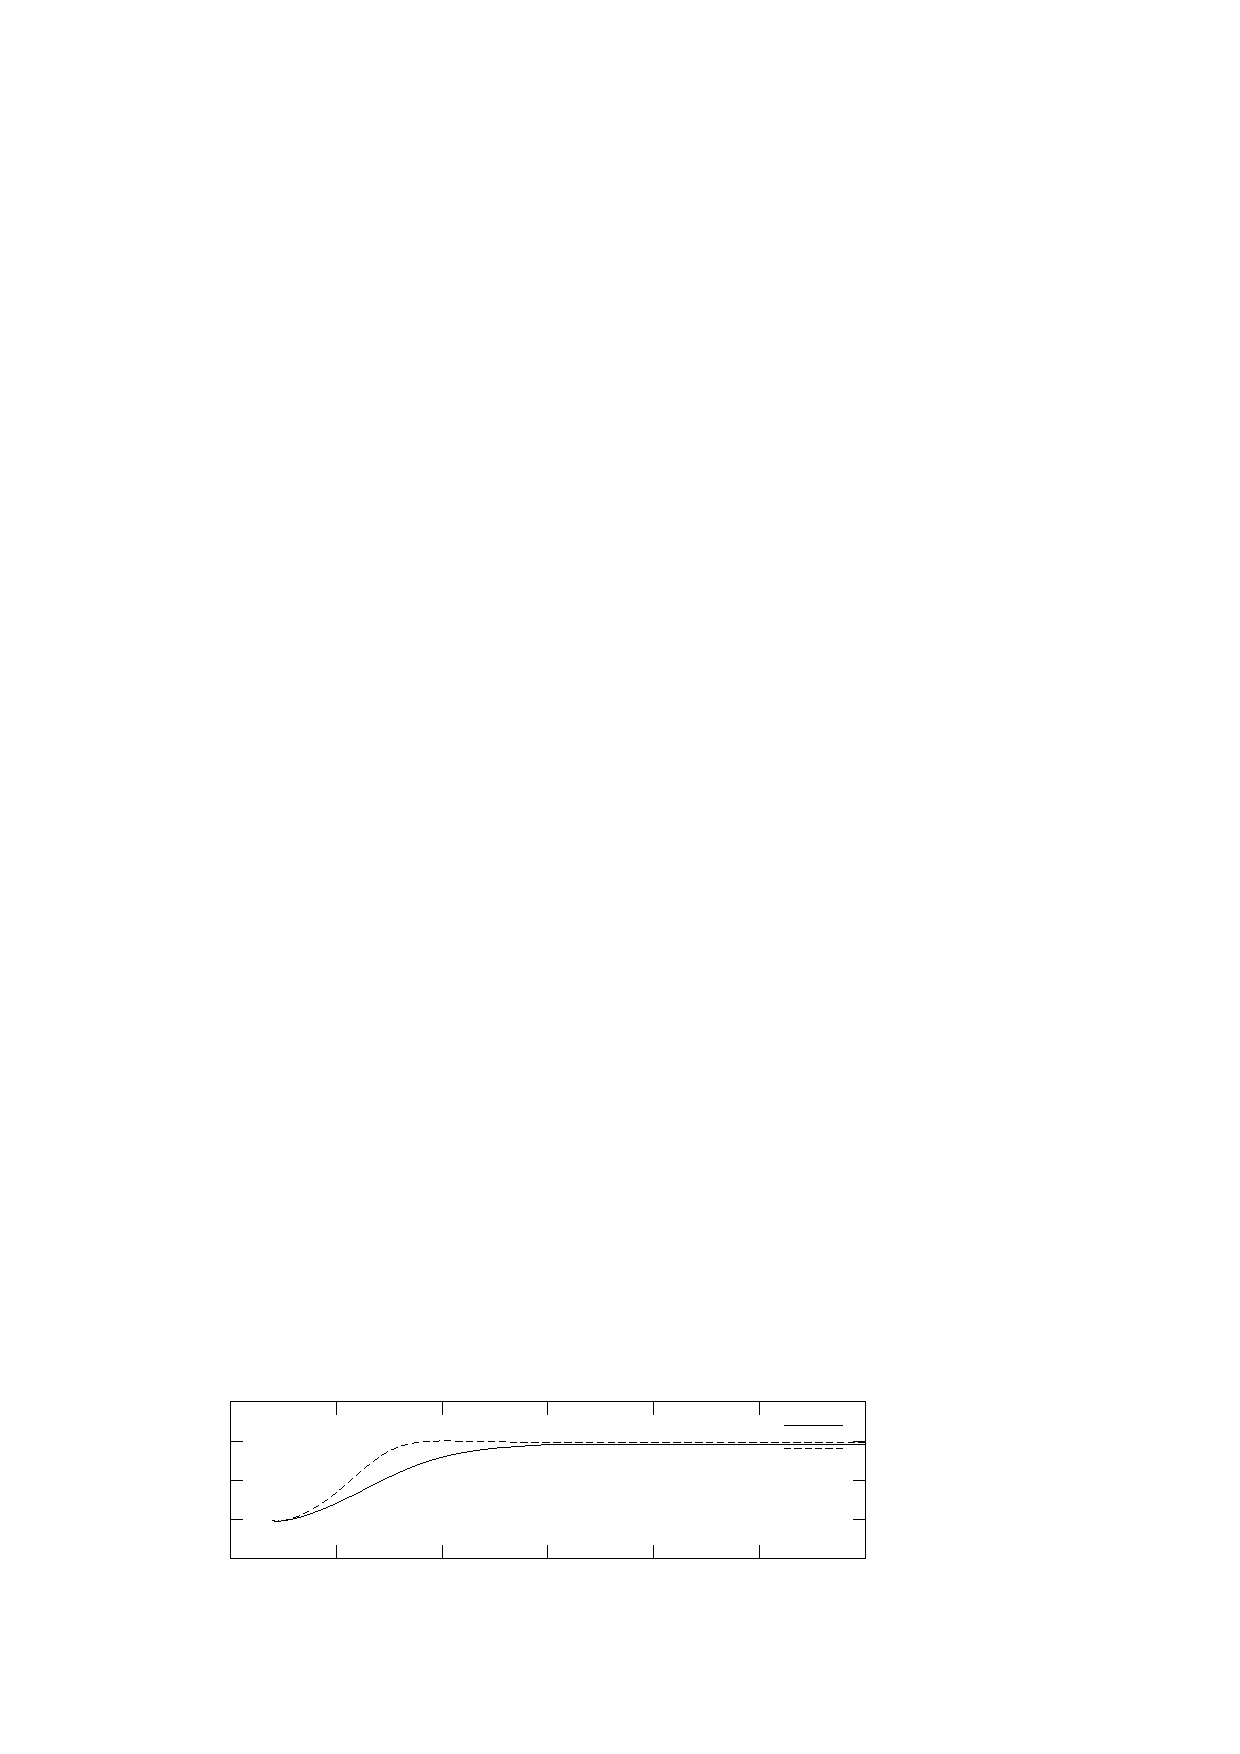
\includegraphics{regimen-1-sedimentacion}%
%\end{picture}%
%\begingroup
%\setlength{\unitlength}{0.0200bp}%
%\begin{picture}(18000,5400)(0,0)%
%\put(1650,1100){\makebox(0,0)[r]{\strut{}0.35}}%
%\put(1650,2038){\makebox(0,0)[r]{\strut{}0.40}}%
%\put(1650,2975){\makebox(0,0)[r]{\strut{}0.45}}%
%\put(1650,3912){\makebox(0,0)[r]{\strut{}0.50}}%
%\put(1650,4850){\makebox(0,0)[r]{\strut{}0.55}}%
%\put(1925,550){\makebox(0,0){\strut{}0.5}}%
%\put(4467,550){\makebox(0,0){\strut{}1.0}}%
%\put(7008,550){\makebox(0,0){\strut{}1.5}}%
%\put(9550,550){\makebox(0,0){\strut{}2.0}}%
%\put(12092,550){\makebox(0,0){\strut{}2.5}}%
%\put(14633,550){\makebox(0,0){\strut{}3.0}}%
%\put(17175,550){\makebox(0,0){\strut{}3.5}}%
%\put(14950,4275){\makebox(0,0)[r]{\strut{}$Re=1.33$}}%
%\put(14950,3725){\makebox(0,0)[r]{\strut{}$Re=2.18$}}%
%\end{picture}%
%\endgroup
%\endinput

%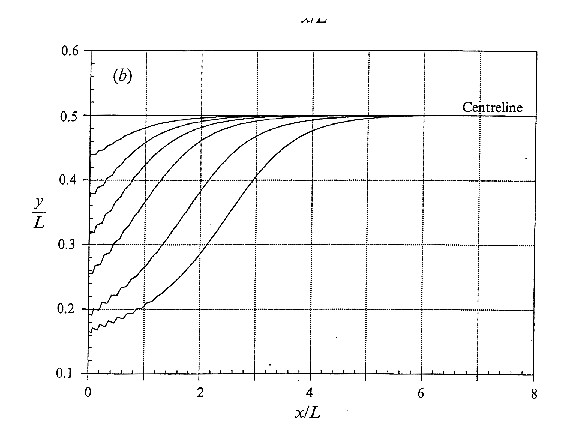
\includegraphics{eps/regimen-1.eps}
\caption{\label{fig:regimen-1-sedimentacion}
Trayectoria de una part'icula s'olida en una cavidad para $Re=1.33$ y $Re=2.18$.
}
\end{figure}
%
\begin{figure}
%%GNUPLOT: LaTeX picture with Postscript
%\begin{picture}(0,0)%
%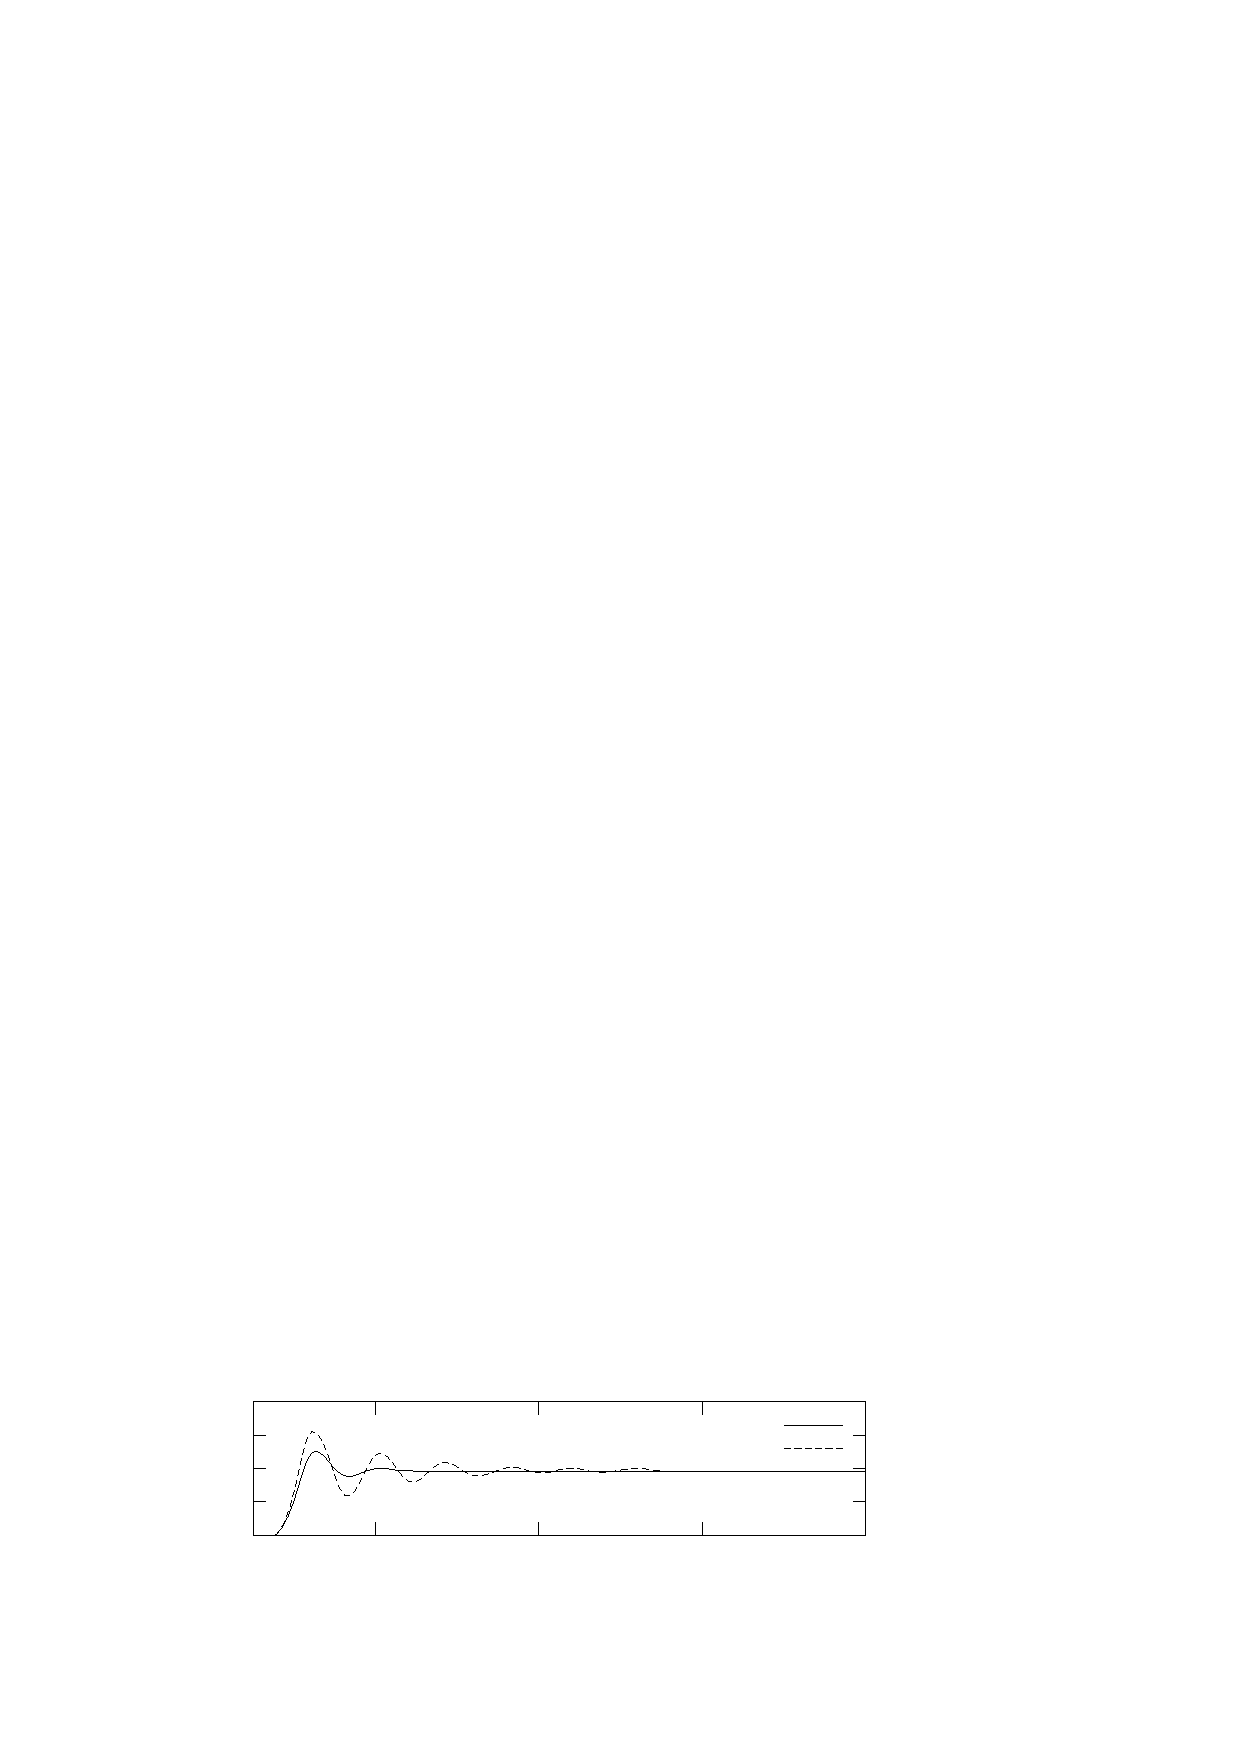
\includegraphics{regimen-2-sedimentacion}%
%\end{picture}%
%\begingroup
%\setlength{\unitlength}{0.0200bp}%
%\begin{picture}(18000,5400)(0,0)%
%\put(2200,1650){\makebox(0,0)[r]{\strut{}0.40}}%
%\put(2200,2450){\makebox(0,0)[r]{\strut{}0.45}}%
%\put(2200,3250){\makebox(0,0)[r]{\strut{}0.50}}%
%\put(2200,4050){\makebox(0,0)[r]{\strut{}0.55}}%
%\put(2200,4850){\makebox(0,0)[r]{\strut{}0.60}}%
%\put(5415,1100){\makebox(0,0){\strut{}2}}%
%\put(9335,1100){\makebox(0,0){\strut{}4}}%
%\put(13255,1100){\makebox(0,0){\strut{}6}}%
%\put(17175,1100){\makebox(0,0){\strut{}8}}%
%\put(550,3250){\rotatebox{90}{\makebox(0,0){\strut{}$y^\ast$}}}%
%\put(9825,275){\makebox(0,0){\strut{}$x^\ast$}}%
%\put(14950,4275){\makebox(0,0)[r]{\strut{}$Re=3.87$}}%
%\put(14950,3725){\makebox(0,0)[r]{\strut{}$Re=6.37$}}%
%\end{picture}%
%\endgroup
%\endinput

\caption{\label{fig:regimen-2-sedimentacion}
Trayectoria de una part'icula s'olida en una cavidad para $Re=3.87$ y $Re=6.37$, correspondientes
al segundo  r'egimen. La particula oscila ligeramente alrededor del centro para finalmente alcanzar una 
posici'on de equilibrio.
}
\end{figure}
%
\begin{figure}
%%GNUPLOT: LaTeX picture with Postscript
%\begin{picture}(0,0)%
%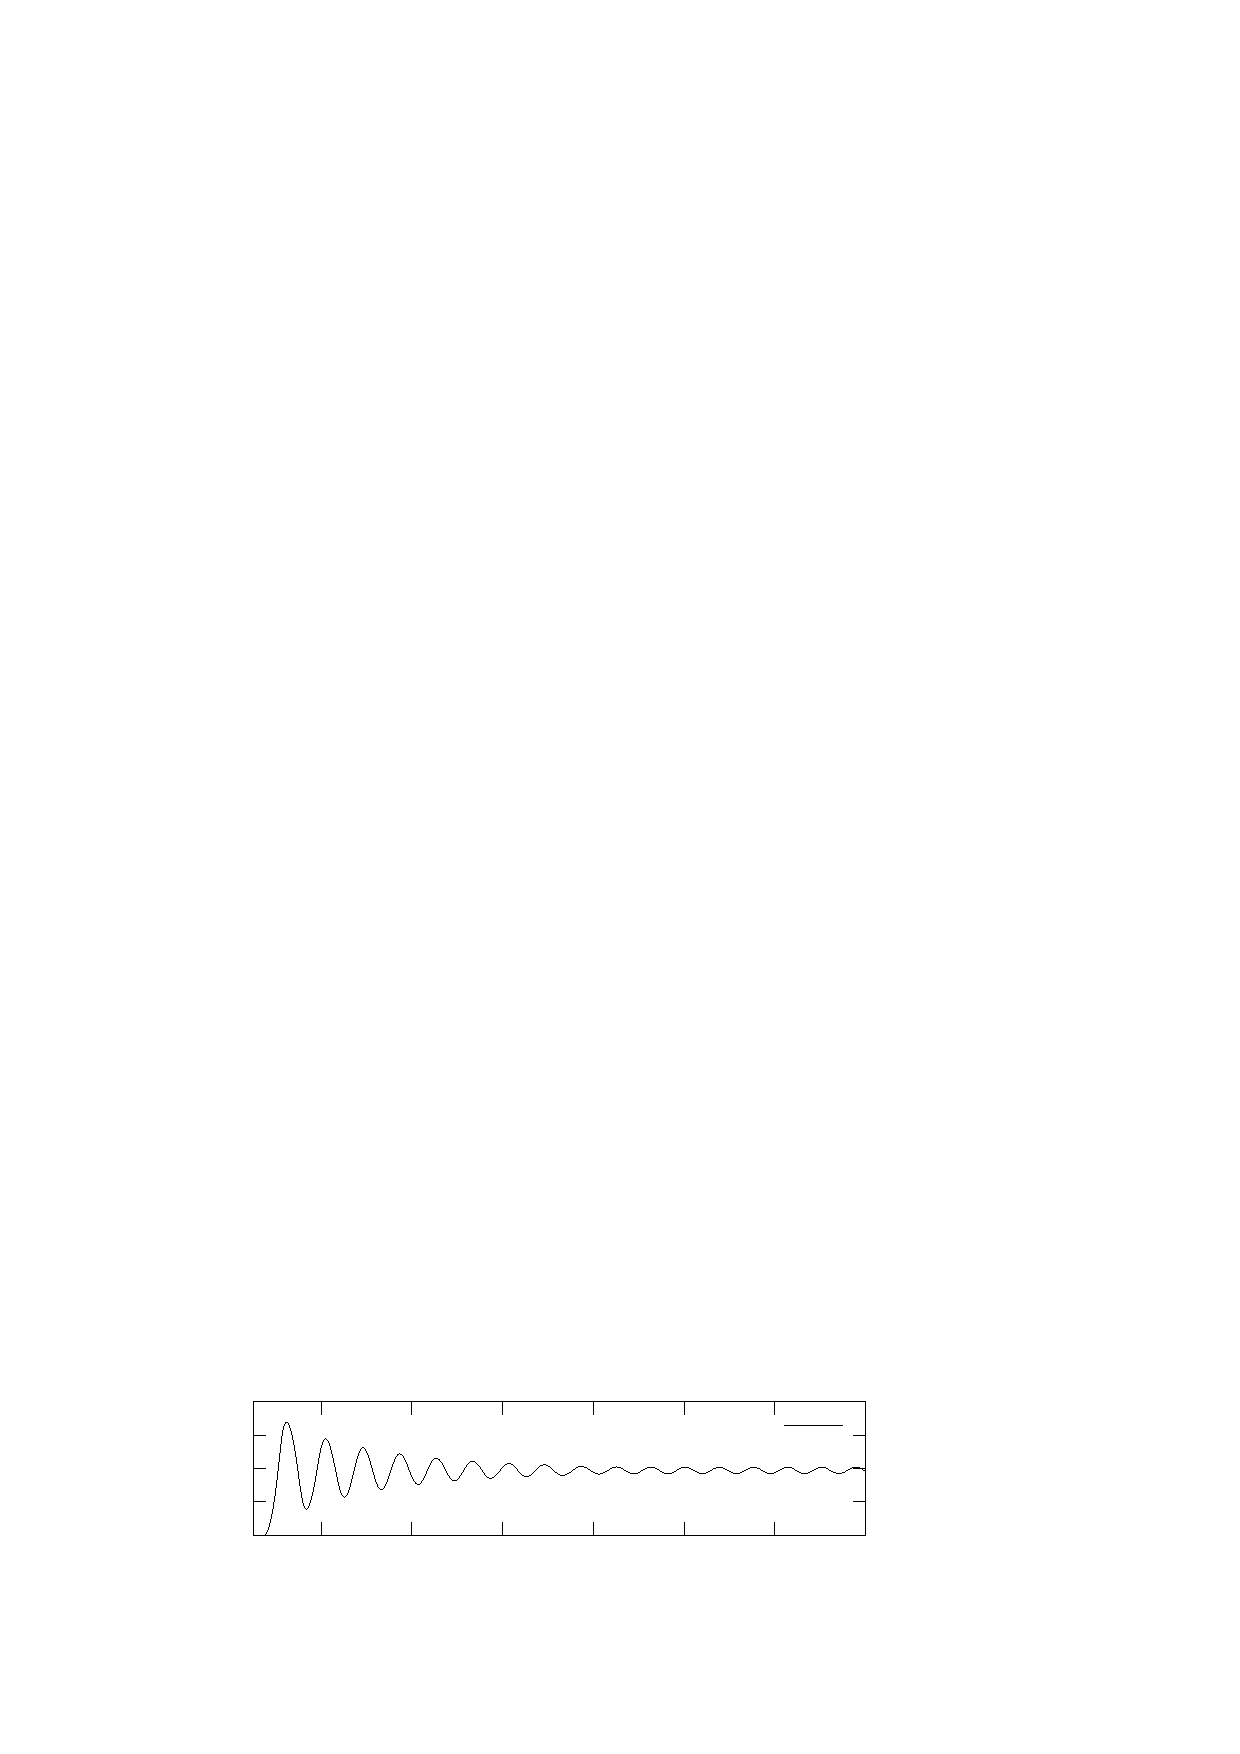
\includegraphics{regimen-3-sedimentacion}%
%\end{picture}%
%\begingroup
%\setlength{\unitlength}{0.0200bp}%
%\begin{picture}(18000,5400)(0,0)%
%\put(2200,1650){\makebox(0,0)[r]{\strut{}0.40}}%
%\put(2200,2450){\makebox(0,0)[r]{\strut{}0.45}}%
%\put(2200,3250){\makebox(0,0)[r]{\strut{}0.50}}%
%\put(2200,4050){\makebox(0,0)[r]{\strut{}0.55}}%
%\put(2200,4850){\makebox(0,0)[r]{\strut{}0.60}}%
%\put(4108,1100){\makebox(0,0){\strut{}2}}%
%\put(6286,1100){\makebox(0,0){\strut{}4}}%
%\put(8464,1100){\makebox(0,0){\strut{}6}}%
%\put(10642,1100){\makebox(0,0){\strut{}8}}%
%\put(12819,1100){\makebox(0,0){\strut{}10}}%
%\put(14997,1100){\makebox(0,0){\strut{}12}}%
%\put(17175,1100){\makebox(0,0){\strut{}14}}%
%\put(550,3250){\rotatebox{90}{\makebox(0,0){\strut{}$y^\ast$}}}%
%\put(9825,275){\makebox(0,0){\strut{}$x^\ast$}}%
%\put(14950,4275){\makebox(0,0)[r]{\strut{}$Re=8.02$}}%
%\end{picture}%
%\endgroup
%\endinput

\caption{\label{fig:regimen-3-sedimentacion}
Trayectoria de una part'icula s'olida en una cavidad para $Re=8.02$, correspondiente
al tercer  r'egimen. La amplitud de la oscilaci'on de la part'icula alrededor del centro
se va reduciendo pero no desaparece.
}
\end{figure}
%
\begin{figure}
%%GNUPLOT: LaTeX picture with Postscript
%\begin{picture}(0,0)%
%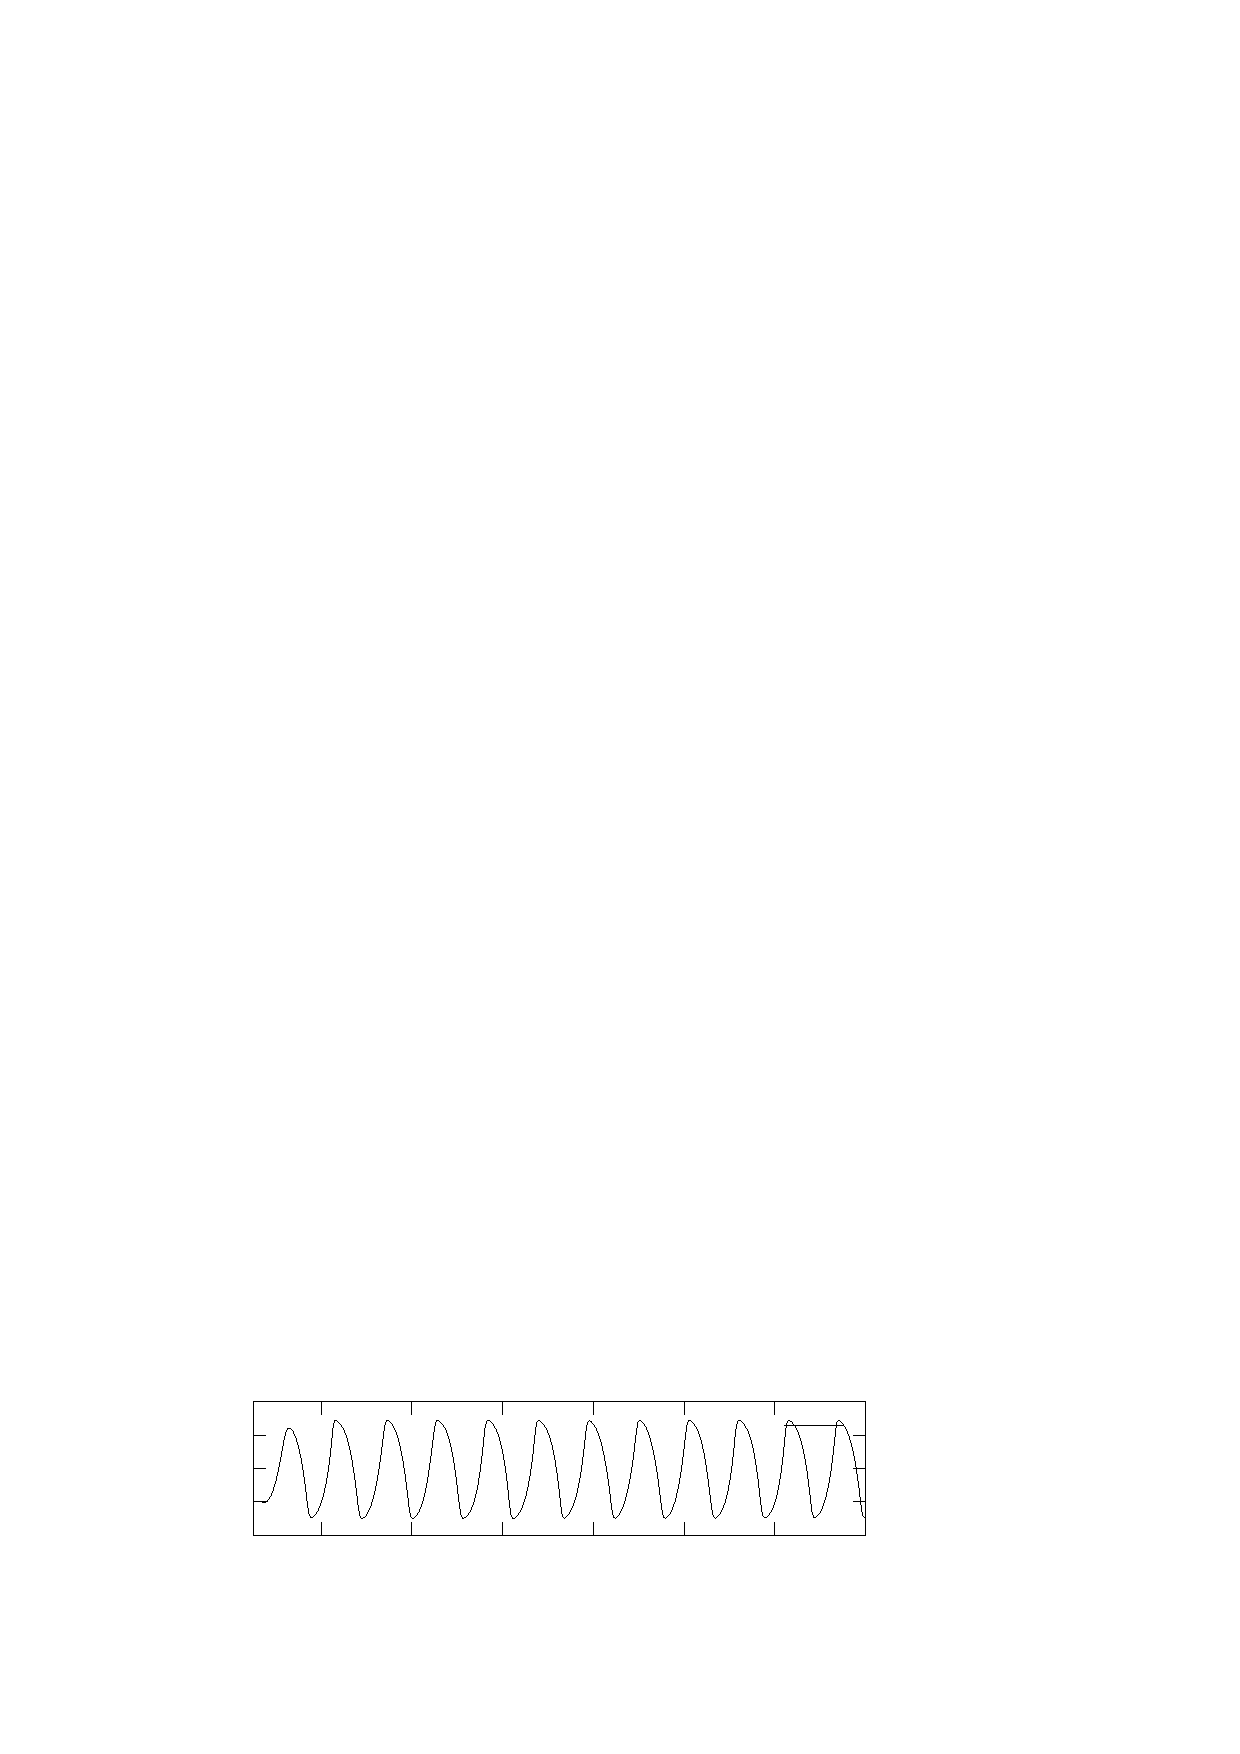
\includegraphics{regimen-4-sedimentacion}%
%\end{picture}%
%\begingroup
%\setlength{\unitlength}{0.0200bp}%
%\begin{picture}(18000,5400)(0,0)%
%\put(2200,1650){\makebox(0,0)[r]{\strut{}0.30}}%
%\put(2200,2450){\makebox(0,0)[r]{\strut{}0.40}}%
%\put(2200,3250){\makebox(0,0)[r]{\strut{}0.50}}%
%\put(2200,4050){\makebox(0,0)[r]{\strut{}0.60}}%
%\put(2200,4850){\makebox(0,0)[r]{\strut{}0.70}}%
%\put(4108,1100){\makebox(0,0){\strut{}2}}%
%\put(6286,1100){\makebox(0,0){\strut{}4}}%
%\put(8464,1100){\makebox(0,0){\strut{}6}}%
%\put(10642,1100){\makebox(0,0){\strut{}8}}%
%\put(12819,1100){\makebox(0,0){\strut{}10}}%
%\put(14997,1100){\makebox(0,0){\strut{}12}}%
%\put(17175,1100){\makebox(0,0){\strut{}14}}%
%\put(550,3250){\rotatebox{90}{\makebox(0,0){\strut{}$y^\ast$}}}%
%\put(9825,275){\makebox(0,0){\strut{}$x^\ast$}}%
%\put(14950,4275){\makebox(0,0)[r]{\strut{}$Re=28.76$}}%
%\end{picture}%
%\endgroup
%\endinput

\caption{\label{fig:regimen-4-sedimentacion}
Trayectoria de una part'icula s'olida en una cavidad para $Re=28.76$, correspondiente
al cuarto  r'egimen. La part'icula oscila fuertemente alrededor del centro manteniendo
su amplitud todo el tiempo.
}
\end{figure}


\section{Conclusiones}

En este ap'endice demostramos que el m'etodo de la ecuaci'on de Boltzmann en redes
es capaz de resolver problemas de fluidos compresibles, que es capaz de reproducir
el movimiento angular de una part'icula s'olida en un flujo Couette. Con el problema
de Couette escogimos el radio de part'icula para realizar las simulaciones num'ericas
de la levitaci'on ac'ustica. El radio escogido $r=9.5$ representa un error
menor al 3\%. Finalmente  simulamos num'ericamente el problema de sedimentaci'on de 
una part'icula en un canal y encontramos  los cuatro reg'imenes previamente reportado. Las
trayectorias para los n'umeros de Reynolds reportados concuerdan con lo 
obtenido num'ericamente. 
Al pasar por estos problemas y obtener datos que coinciden con los reportados en la literatura, nos aseguramos
que el c'odigo con el que realizamos las simulaciones num'ericas del problema de levitaci'on
ac'ustica est'a bien implementado y nos da la confianza para realizar las simulaciones num'ericas.
